\documentclass[%
12pt, %
final, % 
oneside, % 
onecolumn, %  
centertags]{article} % относится к классу article и размер шрифта 12 пунктовб, {article: статья, report: отчеты и диссертации, book: книга, letter: письмо}

% \usepackage{fontspec}
 
% \setmainfont{Times New Roman}

% \documentclass[a4paper, 12pt]{report}

\topmargin= -30pt % насколько сверху будет страница
\textheight= 650pt


\usepackage[utf8]{inputenc} % задает кодировку, utf-8 кодировка, включающая в себя знаки почти всех языков мира
\usepackage[english]{babel} % подключает необходимые языки, основным языком является английский

\selectlanguage{english} % настройки будут на английском, но писать будет на русском

\usepackage{euscript}
\usepackage{supertabular}

\renewcommand{\baselinestretch}{1.0} 

\usepackage[colorlinks=true,linkcolor=blue,unicode=true,urlcolor = blue]{hyperref} %hypered
\usepackage[pdftex]{graphicx} % для графики

\usepackage{amsthm, amssymb, amsmath, amsfonts} % математический пакет, математические шрифты
\usepackage{textcomp}
\usepackage[noend]{algorithmic}
\usepackage[ruled]{algorithm}
\usepackage{lipsum}
\usepackage{indentfirst}
\usepackage{babel}
\usepackage{pgfplots}
\usepackage{setspace}
\usepackage{xcolor}
\usepackage{hyperref}
\usepackage{subfigure}

\setcounter{secnumdepth}{5}
\setcounter{tocdepth}{5}
\newcommand\simpleparagraph[1]{%
  \stepcounter{paragraph}\paragraph*{\theparagraph\quad{}#1}}
\usepackage{listings}
% \usepackage{xcolor}
%\usepackage{minted}

\lstset { %
     language=C++,
     backgroundcolor=\color{black!5}, % set backgroundcolor
     basicstyle=\footnotesize,% basic font setting
}


\linespread{1.0} 
\setlength{\parindent}{2.4em}
\setlength{\parskip}{0.1em}

\pgfplotsset{compat=1.9}
\pgfplotsset{model/.style = {blue, samples = 100}} 
\pgfplotsset{experiment/.style = {red}}

\theoremstyle{plain}
\binoppenalty=10000

\newtheorem{theorem}{Theorem}[section] % theorem

\theoremstyle{definition}
% \newtheorem{definition}{Определение}[subsection]
\newtheorem{definition}{Definition}[subsection]

\theoremstyle{remark}
% \newtheorem{remark}{Замечание}[section]

% \newtheorem{corollary}{Следствие}

% \newtheorem{proposition}{Proposition}

% \newtheorem{example}{Пример}

% \newtheorem{lemma}{Лемма}[section]

\renewcommand*{\proofname}{Proof}

\graphicspath{ {./images/} }


% \usepackage{amsmath,amsfonts,amssymb, setspace}  % Разнообразные математические команды и значки
% \usepackage{indentfirst}     % Отступ в первом абзаце

% \pagestyle{empty}
\usepackage[left=2.5cm, right=1.5cm, top=2.5cm, bottom=2.5cm]{geometry}
\usepackage[medium]{titlesec}
\usepackage{graphicx}
% \graphicspath{ {./images/} }

\begin{document}

	\begin{titlepage} 
		\begin{center}
		\textbf{}\\[2.0cm]
		\LARGE FEDERAL STATE AUTONOMOUS EDUCATIONAL INSTITUTION OF HIGHER EDUCATION \\[0.5cm]
		\Large ITMO UNIVERSITY \\[3cm]
		\LARGE Report\\
		\Large MPI. Assignments $14-15$ \\
		\Large Parallel algorithms for the analysis and synthesis of data \\[4cm]


		\begin{flushright}
		Performed by\\
		Aleksandr Shirokov\\
		J4133c\\
		Accepted by\\
		Petr Andriushchenko

		Deadline: 23.12.21
		\end{flushright}

		\vfill 

		{\Large {St. Petersburg}} \par
		{\Large {2021}}
		\end{center} 
	\end{titlepage}

\tableofcontents
\newpage


\section{Assignments}

\subsection{Assignment 14. MPI. Custom global operations. Custom global function.}

\subsubsection{Formulation of the problem}

Understand the new functions in \textsc{Assignment14.c}.

Create your own global function for finding the maximum element, compare the correctness of execution with the \textsc{MPI\_MAX} operation in the \textsc{MPI\_Reduce()} function

\subsubsection{Example of launch parameters and output. Detailed description of solution}

Code for \textbf{assignment 14} is \href{https:\//github.com/aptmess/parallel_algorithms/blob/master/HT/hw_mpi/Assignment14.c}{here}.

Compilation example: \textsc{mpic++ -o ./cpf/14.o Assignment14.c}

Launch example: \textsc{mpirun --oversubscribe -np 7 ./cpf/14.o}

\begin{center}
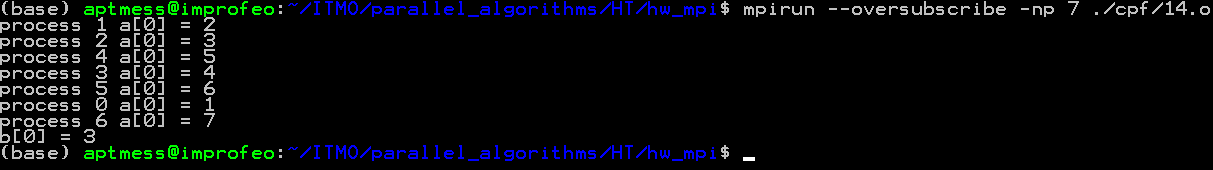
\includegraphics[scale=0.55]{14.png}
\end{center}

Let's move to the the code and explain how it works.

\begin{center}
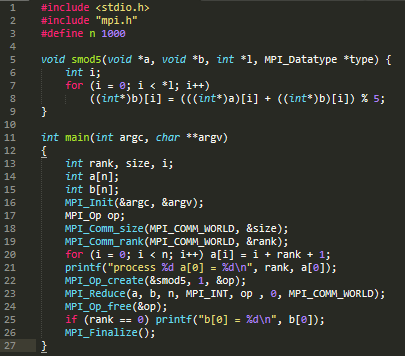
\includegraphics[scale=1.02]{14.code.png}

Assignment14 code
\end{center}

Firstly let's explain how this work code and after that will write the second part of the task. The idea of this program is to show hot to implement user-defined global function for some operations from class \textsc{MPI\_Op}. For each process there is an initialization of array $a$by formula $a[i] = i + rank + 1, i = [1..n]$  where \textsc{rank} is rank of the process and $n$ is amount of processes. For example for $7$ processes $a[0]$ for all processes is $[1..7]$. After that with operation \textsc{MPI\_Op\_create} which allows to create \textsc{MPI\_Op} operation that can be used in reduction operations from an user-defined function and with second parameter $1$ indicatesthat user-defined functon passed is communicative - in our example this function's name is \textsc{smod5} (lines $5-9$). This user-defined function should have such parameters as:

\begin{itemize}
	\item void \textbf{inputBuffer} - A pointer on the buffer providing the inputs of an MPI process. In our example the variable name is $a$;
	\item void \textbf{outputBuffer} - A pointer on the buffer in which write the reduction results. In our example the variable name is $b$;
	\item int \textbf{len} -  The number of elements on which the reduction applies, amount of processes. In our example the variable name is $l$;
	\item MPI\_Datatype* datatype - the datatype of output function
\end{itemize}

Our function \textsc{smod5} implemented a logic - return an residual of sum of elements divided by 5. After that in line $23$ we are using this written function as a reduce function and in the next line function \textsc{MPI\_Op\_free} deallocates an operation handle created with \textsc{MPI\_Op\_create}. As an output in line $25$ we are showing result, which is storted in array $b$. Check if result if correct: $(1 + \ldots + 7) \% 5 = 28 \% 5 = 3$ - as our program shows.

Let's implement a function for finding a maximum.

Code for \textbf{assignment 14 with maximum function} is \href{https:\//github.com/aptmess/parallel_algorithms/blob/master/HT/hw_mpi/Assignment14.1.c}{here}.

Compilation example: \textsc{mpic++ -o ./cpf/14.1.o Assignment14.1.c}

Launch example: \textsc{mpirun --oversubscribe -np 7 ./cpf/14.1.o}

\begin{center}
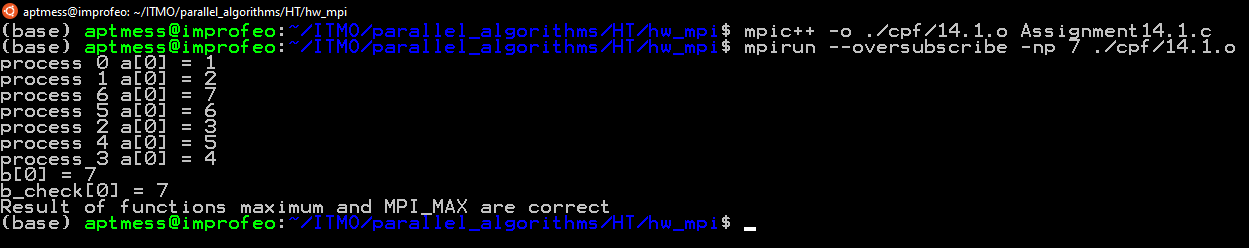
\includegraphics[scale=0.55]{14.1.png}
\end{center}

Let's move to the the code and explain how it works.

\begin{center}
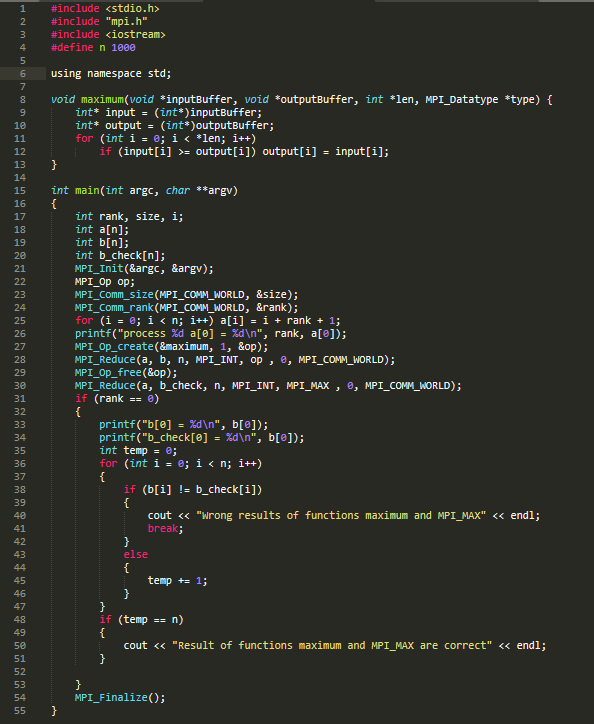
\includegraphics[scale=1]{14.1.code.png}

Assignment14 code
\end{center}

I have implemented function maximum with simple logic for finding maximum (lines $8-13$). At lines $31-53$ i have implemented checking that results of my function is the same as using defined function \textsc{MPI\_MAX} - if every piece of arrays $b$ is equal to appropriate value $b\_check$ then the message that results are correct is displayed, else - that results isn't correct, but it is not our way - our results are correct! The program works correctly.





\newpage
\subsection{Assignment 15. MPI. Operations with communicators. Partitioning the communicator.}

\subsubsection{Formulation of the problem}

Understand the new functions in \textsc{Assignment15.c}.

Append part of code.

\subsubsection{Example of launch parameters and output. Detailed description of solution}

Code for \textbf{assignment 15} is \href{https:\//github.com/aptmess/parallel_algorithms/blob/master/HT/hw_mpi/Assignment15.c}{here}.

Compilation example: \textsc{mpic++ -o ./cpf/15.o Assignment15.c}

Launch example: \textsc{mpirun --oversubscribe -np 5 ./cpf/15.o}

Let's move to the the code and explain how it works.

\begin{center}
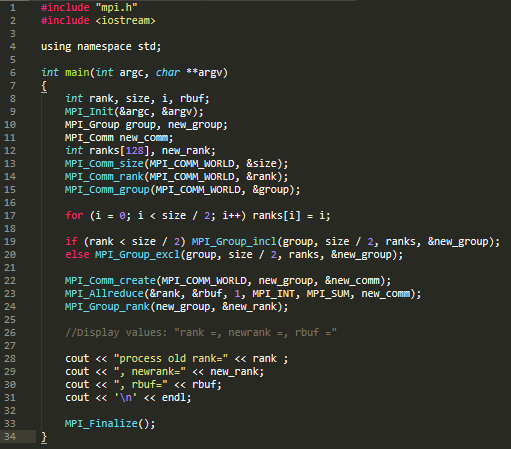
\includegraphics[scale=0.87]{15.code.png}

Assignment15 code
\end{center}

There are some new function in this code. First is \textsc{MPI\_Comm\_group} which accesses the group associated with given communicator, after that there are initialization of array ranks only for $i = \frac{size}{2}$ where $size$ is amount of processes. After that there are functions:

\begin{enumerate}
	\item \textsc{MPI\_Group\_incl} -  (
	\begin{itemize}
		\item IN - MPI\_Group \textbf{group} - group
		\item IN - int \textbf{n} - number of elements in array ranks (and size of newgroup) (integer)
		\item IN - const int \textbf{ranks[]} - ranks of processes in group to appear in newgroup (array of integers)
		\item OUT - MPI\_Group * \textbf{newgroup} - new group derived from above, in the order defined by ranks
	\end{itemize}
	)
	\item \textsc{MPI\_Group\_excl} - Produces a group by reordering an existing group and taking only unlisted members
	(
	\begin{itemize}
		\item IN - MPI\_Group \textbf{group} - group
		\item IN - int \textbf{n} - number of elements in array ranks (integer)
		\item IN - const int \textbf{ranks[]} - array of integer ranks in group not to appear in newgroup
		\item OUT - MPI\_Group * \textbf{newgroup} - new group derived from above, preserving the order defined by group
	\end{itemize}
	)
\end{enumerate}

In our code it means that all processes with this functions are splitted into two groups depend on their's rank - less than $\frac{size}{2}$ goes to the \textsc{new\_group}, more - to the second existing \textsc{group}. For \textsc{new\_group} the new communcator with function \textsc{MPI\_Comm\_create} is creating and after that using function \textsc{MPI\_Allreduce} which combines values from all processes and distributes the result back to all processes - returns sum of rank for \textsc{new\_group} and this rank is written in variable \textsc{new\_rank} as a new rank using function \textsc{MPI\_Group\_rank}. As a results we are displaying information abour rank if process, new rank of process and rbuf as a results of function \textsc{MPI\_Allreduce}.

Let's see an example. Let amount of process be $5$. Then processes of ranks $0, 1$ goes to group \textsc{new\_group} and others are in \textsc{group}. \textsc{rbuf} is a sum of ranks for each group, so for first \textsc{group} it would be $\operatorname{rbuf}=0+1=1$ and for \textsc{new\_group} the result is $\operatorname{rbuf}=2+3+4=9$. \textsc{new\_rank} is new ranks for group \textsc{new\_group}, so the processes with previous ranks $3, 4, 5$ maps appropriate to $0, 1, 2$ in \textsc{new\_group}. For first group ranks are the same.

The results of example are on picture below

\begin{center}
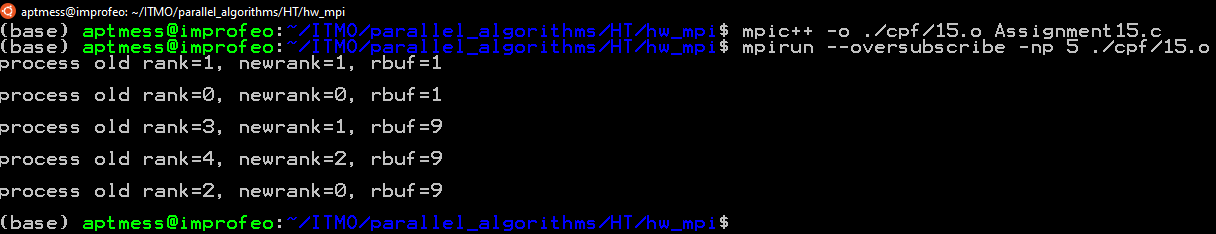
\includegraphics[scale=0.55]{15.png}

Results
\end{center}

The program works correctly!

\subsection{Appendix}

The link to the sourse code which is placed on my \href{https://github.com/aptmess/parallel_algorithms}{github}.


\end{document}